\documentclass[9pt,twocolumn,twoside,lineno]{pnas-new}
% Use the lineno option to display guide line numbers if required.

\usepackage{amsmath}

% PNAS template
% {pnasresearcharticle}=two-column;{pnasmathematics}=one-column mathematics;{pnasinvited}=invited submission
\templatetype{pnasresearcharticle} 

% Title
\title{Estimating populations in data-poor regions using commonly available population-weighted household survey data}

% Author list
\author[a,1]{Douglas R. Leasure}
\author[a]{Claire A. Dooley}
\author[a]{Gianluca Boo}
\author[a]{Édith C. Darin}
\author[a]{Andrew J. Tatem}


% Author affiliations
\affil[a]{WorldPop, Geography and Environmental Science, University of Southampton, Highfield, Southampton SO17 1BJ, UK.}

% Surname for running footer
\leadauthor{Leasure}

% Significance statement
\significancestatement{}

% Author information
\authorcontributions{Leasure, Dooley: methods development, simulations, data analysis; Boo, Darin: field data collection/prep, data analysis; Tatem: project planning and implementation.  All authors contributed to writing.}
\authordeclaration{No conflicts of interest.}
\correspondingauthor{\textsuperscript{1}Corresponding author. E-mail: doug.leasure@gmail.com}

% Keywords
\keywords{demography $|$ international development $|$ Bayesian statistics $|$ household surveys} 

% Abstract 250 words
\begin{abstract}
250 words.
\end{abstract}

% Compile date
\dates{This manuscript was compiled on \today}
\doi{\url{www.pnas.org/cgi/doi/10.1073/pnas.XXXXXXXXXX}}

% Formatting
\begin{document}

\maketitle
\thispagestyle{firststyle}
\ifthenelse{\boolean{shortarticle}}{\ifthenelse{\boolean{singlecolumn}}{\abscontentformatted}{\abscontent}}{}

%-----------------------------------------------%

% Introduction
\dropcap{P}opulation estimates that are accurate and up-to-date are critical for government planning and development projects in low and middle income countries where recent census results may not be available and field surveys designed to collect survey data specifically for population estimation can be logistically challenging.  Household surveys are routinely conducted in these countries, often with national coverage, and they generally enumerate all people in households where surveys are conducted.  There are two challenges preventing these data from being used to estimate population sizes at high resolution: 1) access to sensitive household survey results are protected due to privacy concerns and 2) household surveys generally select sampling locations using a population-weighted sampling scheme to conduct more surveys in high-density urban areas that would be under-represented in a random sample. 

Our objectives are:

\begin{enumerate}
	\item Demonstrate a Bayesian weighted-likelihood model in a simulation environment to correct bias inherent in a weighted sample.
	\item Estimate population sizes in surveyed areas of Kinshasa province in the Democratic Republic of Congo using a random sample collected in the field.
	\item Apply the weighted-likelihood approach to estimate population sizes in surveyed areas of Kinshasa using an independent population-weighted sample collected in the field.
\end{enumerate}

We developed a Bayesian weighted-likelihood model for use with standard household survey data and assessed its performance in simulated and real-world environments.  The population estimates produced here for surveyed areas in Kinshasa province are not intended for uses beyond demonstrating the method.

\subsection*{Results}

\begin{figure}
	\centering
	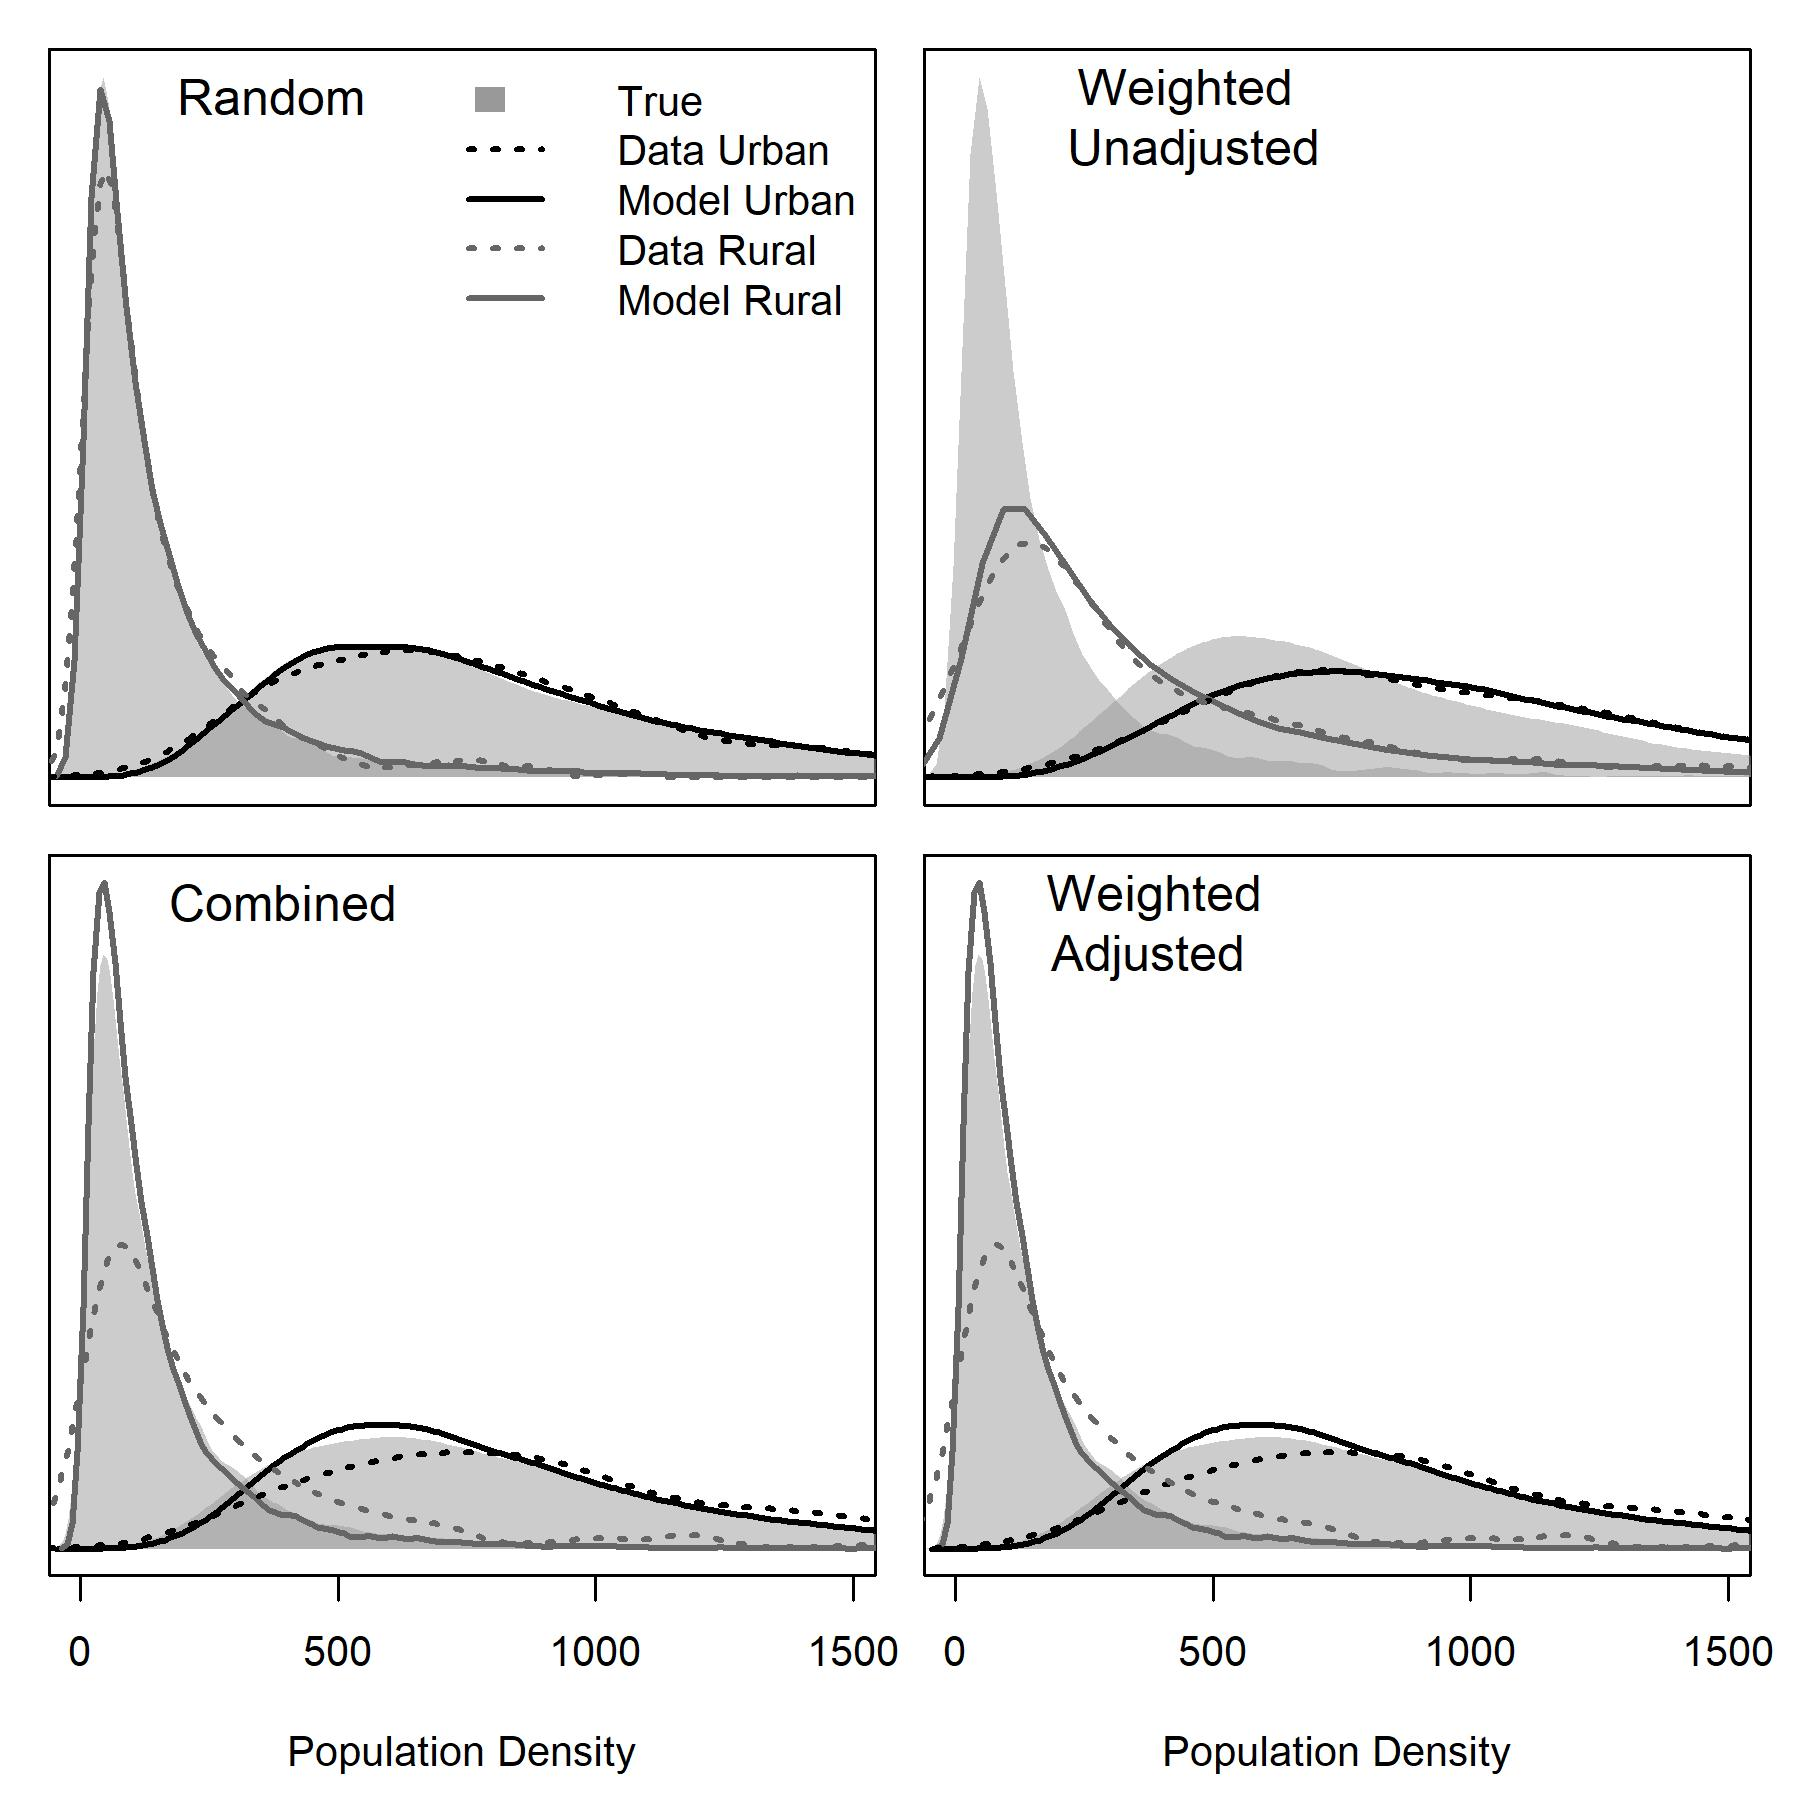
\includegraphics[width=1\linewidth]{sim_model.jpg}
	\caption{Models fit to data from each simulation.}
	\label{fig:sim_model}
\end{figure}

\begin{figure}
	\centering
	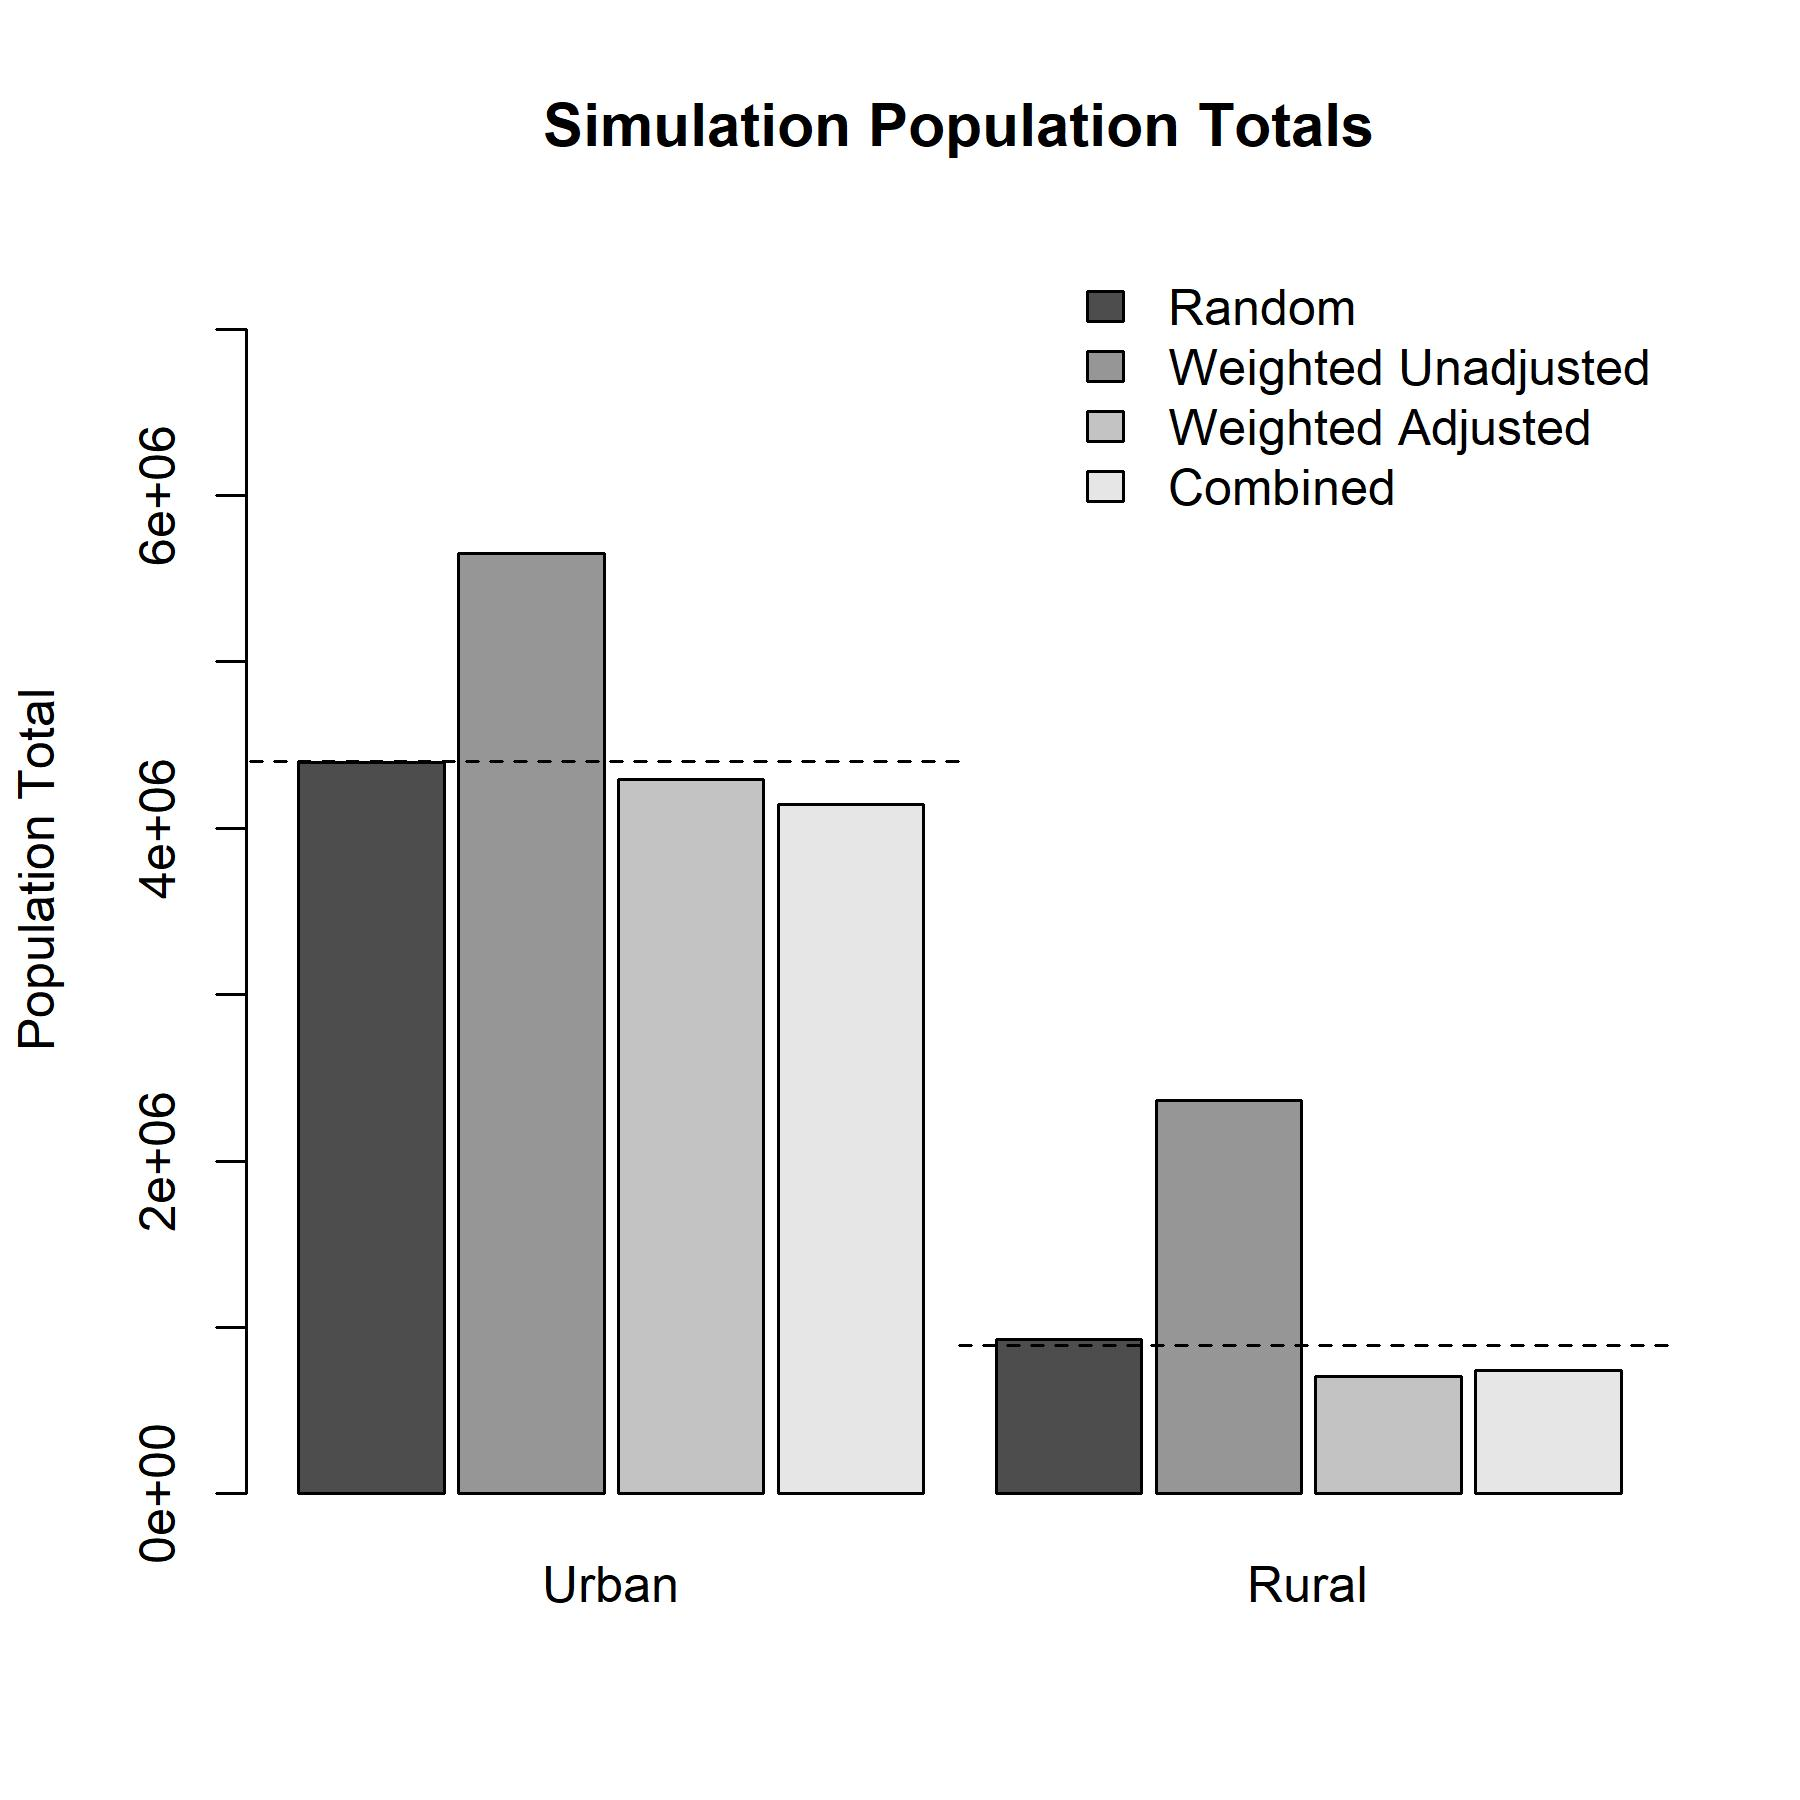
\includegraphics[width=1\linewidth]{sim_totals.jpg}
	\caption{Population totals for urban and rural areas for each simulation. The dashed lines show the actual population totals defined by the simulation for each settlement type.}
	\label{fig:sim_totals}
\end{figure}

\begin{figure}
	\centering
	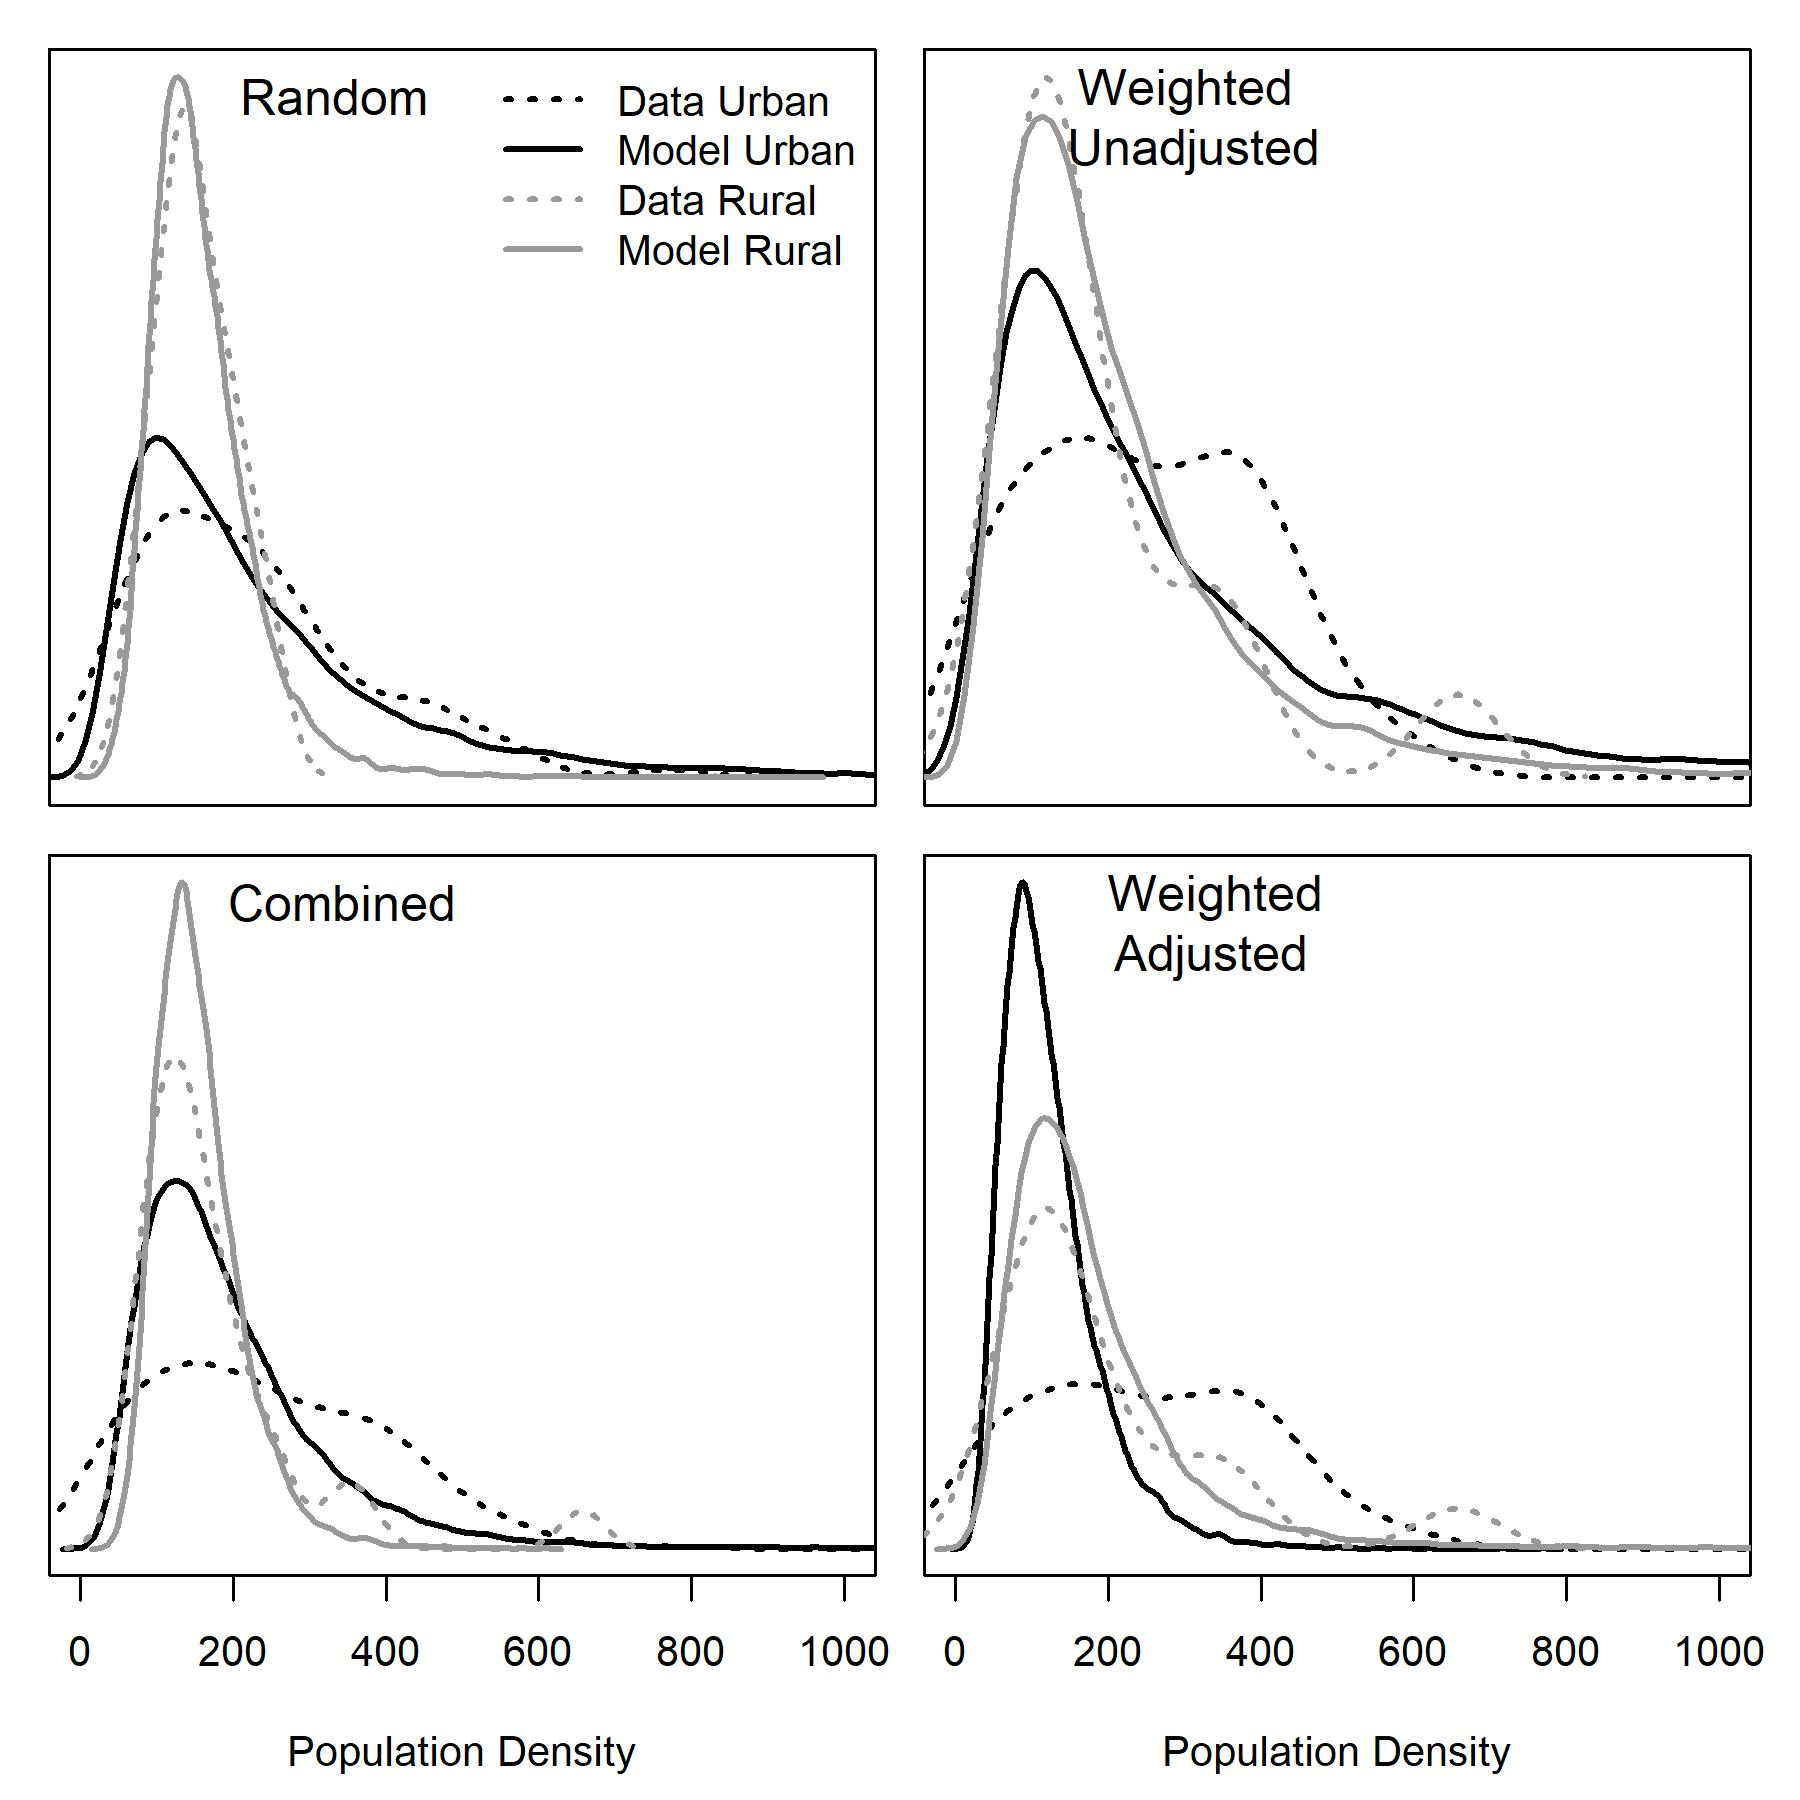
\includegraphics[width=1\linewidth]{drc_model.jpg}
	\caption{Models fit to microcensus data from Kinshasa. The weighted samples from urban areas had two outliers (~1500 people per hectare) that are not shown in the plots.}
	\label{fig:drc_model}
\end{figure}

\begin{figure}
	\centering
	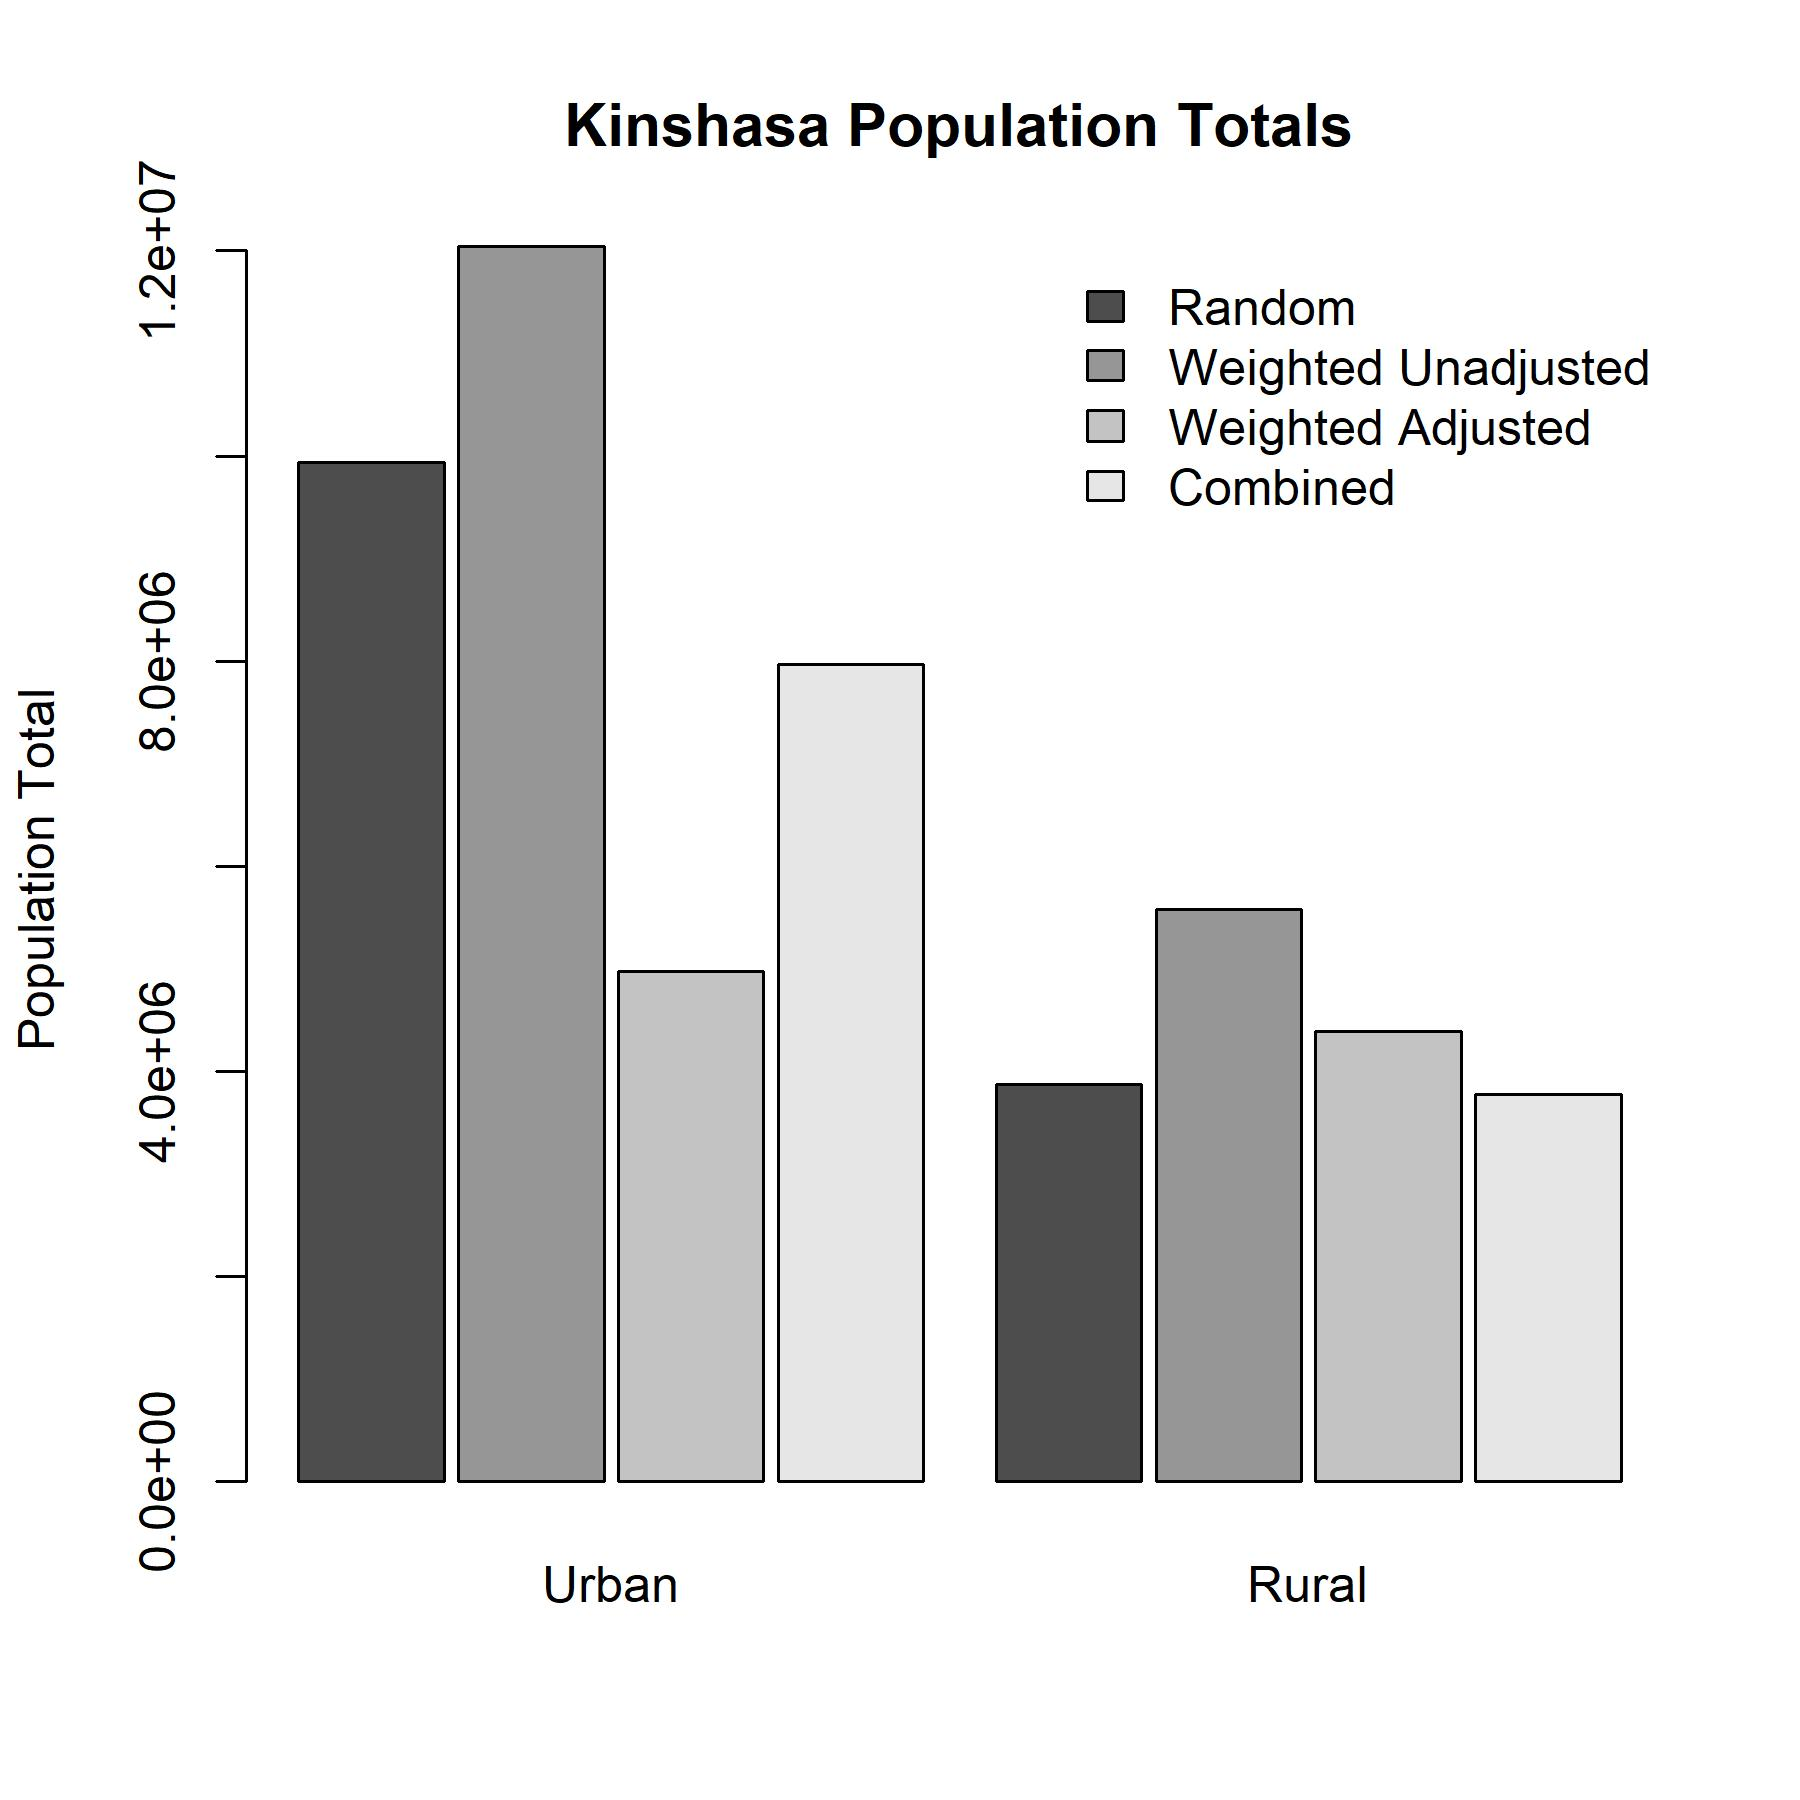
\includegraphics[width=1\linewidth]{drc_totals.jpg}
	\caption{Population totals for urban and rural areas of Kinshasa with random and weighted datasets.}
	\label{fig:drc_totals}
\end{figure}


\subsection*{Discussion}



% Materials and Methods
\matmethods{ 
	
	\subsection{Simulated Data}
	
	Populations were simulated using 10,000 random draws from log-normal distributions to represent a census of a population with people in 10,000 different locations (i.e. each location is a one hectare grid square). Population densities in urban areas were simulated using a median population density of 750 people per hectare with a standard deviation of 500 to parameterise the log-normal distribution.  Populations in rural areas were simulated using a median of 100 and a standard deviation of 250. Half of the locations were urban and half were rural.
	
	These simulated populations were sampled using spatial-random sampling, population-weighted sampling, or both. Samples comprised a total of 1,000 locations that were enumerated in each simulated population (i.e. a 10\% sample from the total population of 10,000 locations). In simulations that included both types of sampling, half of the samples were random and half were population-weighted.  Stratified sampling was implemented so that an equal number of samples were collected from urban and rural areas. Population-weighted sampling used sample weights $w_j$ to define the probabilities for each location $j$ being sampled:
	
	\[ w_j = \frac{N_j}{\sum_{j=1}^{J} N_j } \]
	
	\noindent where $N_j$ is the population size at location $j$, and $J$ is the total number of simulated locations (\textit{i.e.} $J = 10,000$).
	
	Four scenarios were simulated:
	
	\begin{enumerate}
		\item Stratified random sampling with an unweighted model
		\item Stratified weighted sampling with an unweighted model
		\item Stratified weighted sampling with a weighted-likelihood model
		\item Stratified random and weighted sampling with a weighted-likelihood model
	\end{enumerate}  
	
	\subsection{Real Data}
	
	\begin{figure}
		\centering
		
\includegraphics[width=1\linewidth]{doh.png}
		\caption{Map of Kinshasa showing locations of microcensus surveys (random and weighted samples) and settlement types (urban and rural).}
		\label{fig:kinshasa}
	\end{figure}
	
	Two rounds of microcensuses were conducted throughout the Kinshasa province in the Democratic Republic of the Congo (DRC) to collect demographic and socio-economic data for population mapping and estimation (Fig. \ref{fig:kinshasa}). The 2017 microcensus targeted 104 locations using stratified spatial-random sampling \cite{}, while the 2018 microcensus targeted 183 locations using stratified population-weighted sampling \cite{}. Both rounds of microcensuses enumerated all people within the target-locations (i.e. microcensus clusters), each comprising approximatively three hectares of settled area within clearly defined boundaries. 
	
	The stratification adopted in 2017 was based on a morphological settlement classification derived from the LandScanHD database \cite{} consisting of urban, hamlet, and rural settlement types. Microcensus-clusters were then selected from each stratum through spatial-random sampling. The stratification adopted in 2018 was based on a k-means clustering of principal components derived from a set of 16 gridded covariates produced by the WorldPop project \cite{}. This classified each 100 m grid cell as one of three settlement types, labelled as urban, peri-urban, and rural settlement types. Microcensus clusters were then selected using population-weighted sampling, based on the number of people per grid cell estimated by the WorldPop project \cite{}.
	
	In both rounds of microcensuses, a one-stage survey design was implemented, where a listing for each microcensus cluster was created on the same day as the surveys were conducted \cite{}. The surveys produced a roster of individuals in the housing units with basic demographic and socio-economic characteristics (e.g. age, gender, and education). If no respondent was available at the time of the survey, a neighbour could answer in lieu. If no respondent could be identified after three attempts, the size of the housing unit was imputed using the mean value for the microcensus cluster. 
	
	\subsection{Data Analysis}
	
	We used a log-normal weighted-likelihood model to represent the distribution of population densities among locations:
	
	\[ y_i \sim LogNormal( log( \mu_t ), \tau_{t,i} ) \]
	
	\noindent where $y_i$ is the observed number of people at sampled location $i$, and $mu_t$ is the median population size for the settlement type $t$ to which location $i$ belongs. Sample weights $w_i$ were used to calculate model weights $v_i$ to account for the sampling bias:
	
	\[ v_i = \frac{ w_i^{-1} } { \sum_{i=1}^{I} w_i^{-1} }  \]
	
	\noindent where $i$ is a sampled location and $I$ is the total number of sampled locations (i.e. $I = 1,000$).  Model weights are the inverse of sample weights rescaled to sum to one among all sampled locations.
	
	$\tau_i$ is a location-specific estimate of precision (i.e. the inverse of variance; on the log scale) that is dependent on the model weights $v_i$ and a global estimate of precision $\bar{\tau}_t$:
	
	\[ \tau_{t,i} = \bar{\tau}_t v_i \]
	
	We defined the prior distributions of $\mu_t$ and $\bar{\tau}_t$ using uninformative uniform distributions:
	 \[ \mu_t \sim Uniform(0, 5000) \]
	 \[ \bar{\tau}_t \sim Uniform(0, 3) \]
	
	$\bar{\tau}_t$ cannot be used to predict $y$ in new locations where model weights are not available.  So, we used a weighted average of $\tau_{t,i}$ to derive an estimate of precision for each settlement type that can be used for predictions in new locations:
	
	\[ \theta_t = (\frac{\sum_{i=1}^{I_t} v_i \sqrt{\tau_{t,i}^{-1}} }{\sum_{i=1}^{I_t} v_i})^{-2}   \]
	
	\noindent where $I_t$ is the total number of samples from settlement type $t$. The weighted average was calculated based on the standard deviation $\sqrt{\tau_{t,i}^{-1}}$ rather than precision $\tau_{t,i}$ because ?????. This derived estimate of precision was used for making posterior predictions without the need for model weights:
	
	\[ \hat{y}_t \sim LogNormal( log( \mu_t ), \theta_t) \]


	
}

\showmatmethods{}

% Acknowledgements
\acknow{This work was part of the GRID$^3$ project (Geo-Referenced Infrastructure and Demographic Data for Development) funded by the Bill and Melinda Gates Foundation and the United Kingdom Department of International Development.  The project is a collaboration between the WorldPop Research Group at the University of Southampton, the Flowminder Foundation, the United Nations Population Fund (UNFPA), and the Center for International Earth Science Information Network (CIESIN) within the Earth Institute at Columbia University. The authors acknowledge the use of the IRIDIS High Performance Computing Facility, and associated support services at the University of Southampton, in the completion of this work.}

\showacknow{}

% Bibliography
\bibliography{mybib}

\end{document}